\documentclass[letterpaper,11pt]{article}
\usepackage[margin=1in]{geometry}

\usepackage{booktabs}
\usepackage[ruled]{algorithm2e}
\renewcommand{\algorithmcfname}{ALGORITHM}
\SetAlFnt{\small}
\SetAlCapFnt{\small}
\SetAlCapNameFnt{\small}
\SetAlCapHSkip{0pt}
\IncMargin{-\parindent}


\usepackage{multirow}
\usepackage{lmodern}
\usepackage[colorlinks=true,allcolors=teal]{hyperref}
\usepackage[utf8]{inputenc}
\usepackage[T1]{fontenc}
\usepackage{microtype}
\usepackage{dsfont}
\newcommand{\bone}{\mathds{1}}
\usepackage{enumitem}
\setlist{noitemsep}
\setlist[description]{leftmargin=\parindent,labelindent=0pt}
\setlist[itemize]{leftmargin=\parindent,labelindent=0pt}

\usepackage{graphicx}
\usepackage{subcaption}
\usepackage[numbers,sort&compress]{natbib}
\setcitestyle{square}
\usepackage{url}

\usepackage{float}
\usepackage[normalem]{ulem}

\usepackage{tikz}
\usetikzlibrary{positioning, arrows.meta}

\usepackage{amsmath,amsthm,amsfonts}
\usepackage{mathtools,thmtools,thm-restate}
\usepackage{xcolor}
\usepackage[capitalize,nameinlink]{cleveref}
\usepackage{booktabs}
\crefname{demproc}{Process}{Processes}
\crefname{experiment}{Experiment}{Experiments}
\newcommand{\makedemproc}{\SetAlgorithmName{Process}{demproc}{List of Democratic Processes}}
\newcommand{\creflastconjunction}{, and\nobreakspace}

\theoremstyle{plain}
\newtheorem{theorem}{Theorem}
\crefname{theorem}{Theorem}{Theorems}
\newtheorem{lemma}[theorem]{Lemma}
\crefname{lemma}{Lemma}{Lemmas}
\newtheorem{conjecture}[theorem]{Conjecture}
\crefname{conjecture}{Conjecture}{Conjectures}
\newtheorem{corollary}[theorem]{Corollary}
\crefname{corollary}{Corollary}{Corollaries}
\newtheorem{proposition}[theorem]{Proposition}
\crefname{proposition}{Proposition}{Propositions}
\theoremstyle{definition}
\newtheorem{example}[theorem]{Example}
\crefname{example}{Example}{Examples}
\newtheorem{definition}[theorem]{Definition}
\crefname{definition}{Definition}{Definitions}
\crefname{figure}{Figure}{Figures}

\allowdisplaybreaks

\title{Implementation and Cost-Constrained Evaluation of Generative Social Choice on the Abortion Survey Dataset}

 \author{\textbf{Emil Jinu$^1$, Vivek Kumawat$^2$, Sukrut Kulkarni$^3$}}
 \date{\large $^1$Jain University\hspace{.3cm}}




\newcommand{\pg}[1]{\textcolor{black}{#1}}

\definecolor{english}{rgb}{0.0, 0.5, 0.0} 
\newcommand{\dcpadd}[1]{\textcolor{english}{#1}}

\newcommand{\disquery}[2]{\textsc{Disc}(#1, #2)} 
\newcommand{\genquery}[2]{\textsc{Gen}(#1, #2)}

\newcommand{\ttrue}{\mathtt{true}}
\newcommand{\tfalse}{\mathtt{false}}
\newcommand{\emdash}{\,---\,}

\newcommand{\rthlargest}[1]{\mathrm{max}_{(#1)}}

\renewcommand{\theta}{\vartheta}

\DeclareMathOperator*{\argmin}{argmin}
\DeclareMathOperator*{\argmax}{argmax}
\newcommand{\nsubseteq}{\not\subseteq}



% Simpler prompt environment for arXiv
\newenvironment{prompt}{\begingroup\ttfamily}{\endgroup}

% Pretty prompt environment for PDFs
% \usepackage[framemethod=TikZ]{mdframed}
% \definecolor{lightgray}{gray}{0.9}
% \usepackage{letltxmacro}
% \LetLtxMacro\origttfamily\ttfamily
% \DeclareRobustCommand*{\ttfamily}{
%   \origttfamily
%   \hyphenchar\font=`\-\relax
%   \fontdimen3\font=.25em\relax
%   \fontdimen4\font=.167em\relax
%   \fontdimen7\font=.167em\relax
% }
% \newmdenv[
%   backgroundcolor=lightgray,
%   font=\ttfamily\footnotesize,
% ]{prompt}

\usepackage{soul}

\providecommand{\tightlist}{
  \setlength{\itemsep}{0pt}\setlength{\parskip}{0pt}}

\makeatletter
\newcommand{\removelatexerror}{\let\@latex@error\@gobble}
\makeatother


\begin{document}


\maketitle

\begin{abstract}
The mathematical study of voting, \emph{social choice theory}, has traditionally been limited to choices among a few predetermined alternatives, and does not directly address open-ended decisions such as collectively selecting a textual statement. \emph{Generative social choice} addresses this gap by combining the rigor of social choice theory with the ability of large language models to generate text and extrapolate preferences. In this work, we implement a cost-constrained generative social choice pipeline on the original abortion-policy opinion survey, using the locally served open-weight model \texttt{qwen3:8b} to answer discriminative and generative queries. Participant opinions are summarised, embedded, and organised into nearest-neighbour groups, and a budgeted statement-selection algorithm constructs a slate under a 500-word limit. In an experiment with 100 participants, the pipeline evaluated 251 candidate statements, selected 18 statements representing 79 participants, and used 359 of the 500 available words. The discriminative queries produced 4603 agreement scores on a scale of 1--6, and the resulting slate was examined for coverage, lexical diversity, and budget utilization. These results demonstrate a working end-to-end implementation of cost-constrained generative social choice with an open-weight local model, and establish a practical basis for LLM-based opinion summarization.
\end{abstract}



\section{Introduction}

\subsection{Research Problem}

Voting is a central mechanism through which groups, national electorates, legislatures, and committees, make collective decisions. The mathematical foundation for such decisions is provided by \emph{social choice theory}, which studies how voting rules aggregate individual preferences into a collective outcome~\citep{aziz2017jr}. Classical social choice settings, however, assume a \emph{small, predetermined set of alternatives}: voters express preferences over a fixed list of candidates, and a rule selects an outcome from that list.

Many real policy questions are too nuanced for this template. Issues such as abortion policy, climate change, and electoral reform admit a very large space of possible positions, and a short fixed list of options can omit the viewpoints that best capture a population's opinions. Open-ended democratic input is therefore increasingly sought through deliberative processes and online participation platforms~\citep{fish2026gsc,boehmer2025nextgen}. Such processes can surface detailed opinions, but deliberation alone scales poorly and provides no formal guarantee that the resulting summary represents all substantial segments of a population~\citep{fish2026gsc}.

The research problem addressed in this work is the following: \emph{how can free-form opinions from a population be distilled into a concise slate of statements that reflects the diversity and relative prevalence of those opinions, while respecting a limit on the total length of the slate?} Traditional social choice methods cannot generate new alternatives and treat all statements as having equal cost~\citep{boehmer2025nextgen}, while unconstrained LLM summarisation lacks a principled notion of representation. Generative social choice was proposed to bridge this gap by combining representation axioms from social choice with the text-generation and preference-extrapolation capabilities of large language models~\citep{fish2026gsc}. In this report, we study a practical, cost-constrained instance of that problem: using the 100-participant abortion-policy survey from the original GSC study, we implement the query-based statement-selection process with a locally hosted LLM and examine the resulting slate under a fixed word budget.

\subsection{Importance of the Research}

Generative social choice is important because it extends collective decision-making to questions for which the set of possible answers cannot be listed in advance. Two properties of large language models make this extension possible, and a third practical consideration makes it deployable. \smallskip

\begin{itemize}
\item \textit{Unforeseen alternatives.}
In classical social choice the set of alternatives is fixed before voters are consulted, so any option that is not listed cannot be selected. LLMs can instead \emph{generate} new statements that capture common ground between participants, allowing the outcome space to include positions that nobody proposed explicitly~\citep{fish2026gsc,boehmer2025nextgen}. \smallskip

\item \textit{Preference extrapolation.}
Voters normally express preferences only over the alternatives they are shown. When alternatives are generated dynamically, preferences over them must be inferred. LLMs allow participants to state their views in ordinary language and let the system act as a proxy that predicts how well a new statement matches those views~\citep{fish2026gsc}. \smallskip

\item \textit{Cost-aware slates.}
Real consumers of a summary have limited attention. Modelling statement length as a cost and imposing a total word budget makes the resulting slate both readable and comparable across runs, and connects the problem to participatory budgeting~\citep{boehmer2025nextgen}. \smallskip

\item \textit{Accessible implementation.}
Locally served open-weight models make the full pipeline reproducible without reliance on a proprietary API. We implement the queries with \texttt{qwen3:8b}~\citep{yang2025qwen3} served through Ollama~\citep{ollama2026}, so the same experiment can be rerun on ordinary local hardware.
\end{itemize}

For the abortion-policy survey studied here, this means that a short slate can be constructed directly from free-text opinions rather than from a preselected menu of statements, and that the resulting slate can be examined for participant coverage, statement diversity, and budget use.


\subsection{Research Objectives}

The generative social choice framework separates the design of a democratic process into a theoretical component, which gives representation guarantees under ideal queries, and an empirical component, which implements those queries with a language model~\citep{fish2026gsc}. This work contributes to the empirical component. Its objectives are: \smallskip

\begin{enumerate}
\item To examine how large language models can support open-ended collective decision-making by generating candidate statements and estimating participant agreement directly from free-text opinions~\citep{fish2026gsc}. \smallskip

\item To implement a cost-constrained statement-selection process on the original abortion-policy survey dataset and to study how an explicit word budget shapes the size and content of the resulting slate~\citep{boehmer2025nextgen}. \smallskip

\item To instantiate the discriminative and generative queries with a locally served open-weight model, \texttt{qwen3:8b}~\citep{yang2025qwen3}, and to characterise its behaviour in terms of agreement scores, generation success, and statement quality. \smallskip

\item To evaluate the resulting slate along several complementary dimensions, participant representation, statement diversity, approval-score distribution, resource use and to relate the findings descriptively to the results reported in the generative social choice literature~\citep{fish2026gsc,boehmer2025nextgen}.
\end{enumerate}

These objectives yield an end-to-end empirical study of LLM-based opinion summarisation under a word budget using an accessible local model.


\section{Literature Review}

\subsection{Existing Research}

Social choice theory studies how individual preferences are aggregated into collective decisions, with classical results developed for a fixed and typically small set of alternatives. In approval based committee elections, a substantial literature defines proportionality through justified representation (JR) and extended justified representation (EJR), which require that sufficiently large and cohesive groups of voters obtain representation in the elected committee~\citep{aziz2017jr}. Statement selection can be viewed as such an election when statements play the role of candidates and agreement between a participant and a statement plays the role of an approval vote~\citep{fish2026gsc}.

Generative social choice was introduced to move beyond a fixed candidate set. Fish et al.~\citep{fish2026gsc} treat every well formed statement as a potential candidate and access this space through two queries. A discriminative query predicts the utility that a participant assigns to a statement, while a generative query produces a statement tailored to a group of participants. They formulate balanced justified representation (BJR), design a democratic process that satisfies it under ideal queries, and then implement those queries with a large language model in a study of 100 participants on abortion policy. Their experiments show that language model queries can approximate the idealised queries and produce a slate that participants judge as highly representative.

Boehmer et al.~\citep{boehmer2025nextgen} extend this framework in two directions that are central to the present work. First, they assign each statement a cost equal to its length in words and impose a total budget on the slate, which connects the problem to participatory budgeting and removes the need to fix the number of statements in advance. Second, they allow the queries to be approximate, with error parameters for discriminative and generative answers, and prove a cost aware form of BJR that degrades with those errors. Their PROSE implementation uses language models to answer both query types and reports improvements over zero shot, clustering, and unit cost baselines on drug review and deliberation datasets.

The language model used in this report belongs to the Qwen3 family of open weight models, which include dense and mixture of expert variants together with thinking and non thinking modes~\citep{yang2025qwen3}. Serving such a model locally through Ollama~\citep{ollama2026} allows the full query pipeline to run without a proprietary API, which is the setting adopted here.

\subsection{Research Gap}

The representation literature provides strong axioms such as justified representation and extended justified representation for approval based committee elections~\citep{aziz2017jr}, and balanced justified representation for statement selection~\citep{fish2026gsc}. The cost constrained extension further develops a representation guarantee that tolerates approximate queries and statements of varying word length~\citep{boehmer2025nextgen}. These results specify what a representative slate should satisfy under ideal or bounded error queries, but they do not by themselves describe how such a pipeline behaves when it is instantiated with a particular locally served model and applied to the original abortion policy survey.

Three practical questions therefore remain open. First, how does a cost constrained statement selection process behave on the original 100 participant abortion policy dataset, rather than on drug review or city deliberation data? Second, can the two query types be implemented entirely with a local open weight language model such as \texttt{qwen3:8b}\citep{yang2025qwen3} served through Ollama\citep{ollama2026}, while preserving the validation and word budget checks that the process requires? Third, what does the resulting slate look like when it is examined from several angles at once, including agreement scores, participant coverage, statement diversity, budget use, and runtime?

This report addresses these questions by implementing the query based, budget constrained process on the abortion policy survey and by evaluating the resulting slate from the recorded run data. The contribution is empirical: it connects the formal design of representative statement selection to a concrete, locally hosted implementation and a multi measure evaluation of its output.

\section{Dataset Description and Preprocessing}

\subsection{Dataset Source}

The dataset used in this work is the abortion-policy opinion survey released with the generative social choice study of Fish et al.~\citep{fish2026gsc}. In the original study, 100 US residents were recruited through Prolific in August 2024, stratified to reflect the US population in terms of gender and voting behaviour in the 2020 presidential election. Participants answered four open questions about abortion, wrote a self-contained three-sentence statement of their own position, and rated five example statements on a seven-point agreement scale with written explanations~\citep{fish2026gsc}. The full participant responses were made publicly available as the GSC survey dataset~\citep{gsc_survey_data}.

The same material is organised into a generation sample and a separate validation sample. The experiments reported here use the generation sample, which contains 100 participant records. The original study used the generation sample to construct the slate and a separate validation sample to evaluate it~\citep{fish2026gsc}. The same survey data has also been discussed in subsequent work on cost-constrained generative social choice~\citep{boehmer2025nextgen}, which makes the present use directly comparable to the published studies.

\subsection{Dataset Characteristics}

The generation sample consists of 100 participants, identified in the cleaned dataset as \texttt{generation1} through \texttt{generation100}. Each participant contributed free-text answers to four survey questions about abortion, a self-written three-sentence statement of their own position, and ratings of five example statements on the seven-point scale used in the original study~\citep{fish2026gsc,gsc_survey_data}. For the experiments reported here, the preserved free-text responses are the source material for the participant summaries used by the queries.

The cleaned sample contains 100 records, each with a participant identifier and a text field that preserves that participant's responses in order. The responses provide detailed natural-language descriptions of individual viewpoints, which makes the dataset suitable for summarisation and preference extrapolation~\citep{fish2026gsc}. The public availability of the data also makes the setting reproducible~\citep{gsc_survey_data}.

The dataset is therefore well suited to this task: it provides detailed natural-language opinions for a medium-sized population, it is publicly available~\citep{gsc_survey_data}, and it has been used in prior generative social choice experiments~\citep{fish2026gsc,boehmer2025nextgen}.

\subsection{Data Preprocessing}

The cleaned generation sample was validated before use. The dataset contains exactly two columns, a participant identifier and a text field, with 100 unique non-empty identifiers and 100 non-empty text records. For each participant, the text field is parsed into five preserved response blocks using a pattern that matches each survey response in order. These blocks are checked against the long-text responses in the original survey export, so that the cleaned file preserves the original wording while removing survey metadata~\citep{fish2026gsc,gsc_survey_data}. Identifiers are checked for duplicates and empty values, and every response block must match the corresponding original text, which ensures that the cleaned file used in the experiments is a faithful copy of the public data.

\subsection{Dataset Creation and Transformation}

The original survey responses are transformed into the inputs required by the statement-selection process in three stages. First, each participant's five free-text responses are condensed into a structured summary, giving a compact and comparable description of that participant's views. All 100 summaries were generated successfully and are used as the participant text in both query implementations~\citep{fish2026gsc,boehmer2025nextgen}. Each summary records an overall opinion summary together with policy positions, conditions or restrictions, supporting examples, and background information.

Second, the summaries are encoded as 1024-dimensional vectors with the \texttt{qwen3-embedding:0.6b} model~\citep{yang2025qwen3} served through Ollama~\citep{ollama2026}. Cosine distance between these vectors is used to form four overlapping nearest-neighbour groups: two groups of five participants and two groups of ten participants. These groups define the coalitions passed to the generative query in each round of the algorithm~\citep{boehmer2025nextgen}.

Together, the participant summaries and the embedding-based groups form the transformed dataset used by the query implementations in the statement-selection process.

\section{Proposed Methodology}

\subsection{Proposed Model}

The proposed model follows the query based formulation of generative social choice~\citep{fish2026gsc}. A population of $n=100$ agents, denoted by $N$, is associated with a utility function $u_i$ over a universe of well formed statements $\mathcal{U}$. Instead of enumerating $\mathcal{U}$, the process accesses it through two queries. A discriminative query $\disquery{i}{\alpha}$ returns the utility that agent $i$ assigns to statement $\alpha$; in this implementation the answer is an integer from 1 to 6 produced by the language model. A generative query $\genquery{S}{\ell,x}$ returns a statement of cost at most $x$ that is approved at level $\ell$ by the largest number of agents in a coalition $S$.

Following the cost aware extension of~\citet{boehmer2025nextgen}, the cost $c(\alpha)$ of a statement is its length in words, measured by a whitespace token count, and the process is constrained by a total budget $B=500$ words. The output is a slate $W$ of statements whose total cost does not exceed $B$. Each selected statement is assigned a balanced number of supporters, computed as $\lceil c(\alpha)\,n/B\rceil$, so that the share of the slate devoted to a statement reflects the size of the group it represents. This assignment rule instantiates the cost aware form of balanced justified representation~\citep{boehmer2025nextgen,aziz2017jr}.

The model is empirical: the two queries are answered by \texttt{qwen3:8b} rather than by exact oracles, and the resulting utilities are estimates of participant agreement. The remaining subsections describe how the queries, the selection algorithm, and the validation checks are performed in code.

\subsection{Model Architecture}

The implementation is organised as a pipeline of four interacting components: participant representation, the two query modules, the statement-selection controller, and the recorded run state.

\begin{itemize}
\item \emph{Participant representation.}
Each participant's free-text responses are summarised and embedded with \texttt{qwen3-embedding:0.6b}~\citep{yang2025qwen3} through Ollama~\citep{ollama2026}. Cosine distance between the resulting 1024-dimensional vectors is used to form four overlapping nearest-neighbour groups, two of size five and two of size ten, which supply the coalitions for the generative query~\citep{boehmer2025nextgen}. \smallskip

\item \emph{Discriminative query.}
The discriminative query maps an agent and a statement to an integer utility from 1 to 6. It wraps a \texttt{FastAgent} with an Ollama backed scorer that requests a single JSON score and retries up to three times if the response is invalid. The score scale is defined in the agreement prompt, and each participant-statement pair is cached so that repeated calls return the same value~\citep{fish2026gsc}. \smallskip

\item \emph{Generative query.}
The generative query maps a coalition, a target approval level, and a word limit to one candidate statement. It wraps a \texttt{FastGenerator} using the high detail prompt, passes only participant summaries as context, and accepts a statement only if it is a single \texttt{<opinion>} block that fits the word limit. Up to three generation attempts are allowed before the candidate is recorded as a failure~\citep{boehmer2025nextgen}. \smallskip

\item \emph{Statement-selection controller.}
The controller runs the budgeted selection process over utility levels $6,5,\dots,1$ and cost limits $1,2,\dots,500$. In each round it generates candidates from every group for every target level, scores them with the discriminative query, and chooses the statement with the largest number of supporters. A statement is added only when its supporters meet $\lceil c(\alpha)\,n/B\rceil$, after which the assigned supporters are removed and the word budget is reduced. Every candidate, selection, and budget update is recorded so that the full slate can be examined later~\citep{boehmer2025nextgen}.
\end{itemize}

\begin{figure}[htb]
\centering
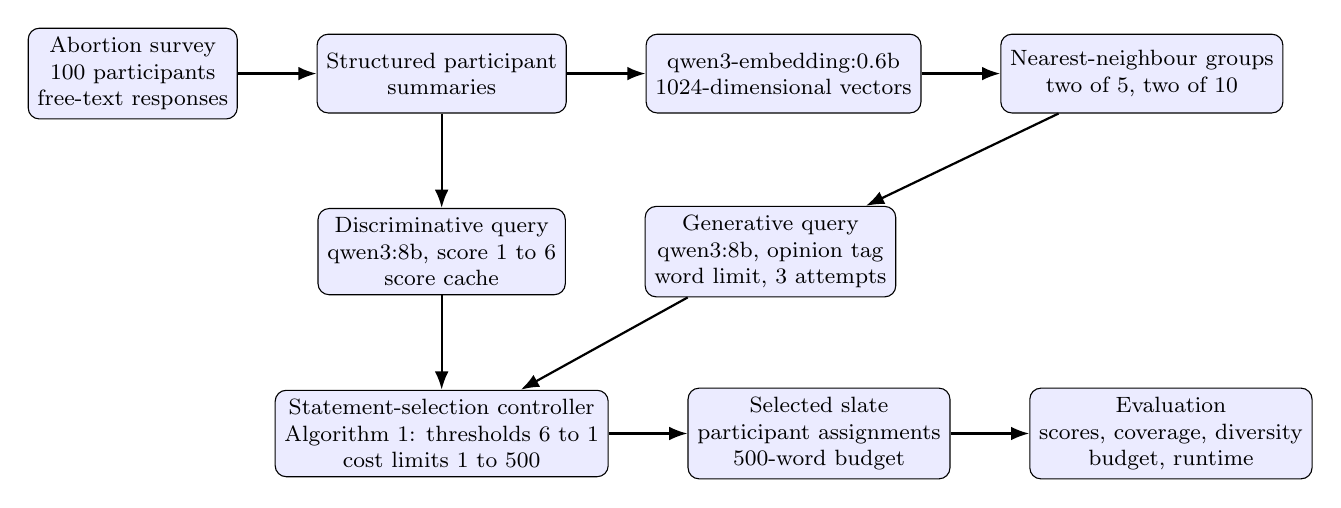
\begin{tikzpicture}[
  box/.style={draw, rounded corners, fill=blue!8, align=center, minimum height=1.0cm, font=\footnotesize},
  arr/.style={->, >=Latex, thick}
]
\node[box] (survey) {Abortion survey\\100 participants\\free-text responses};
\node[box, right=1.0cm of survey] (summary) {Structured participant\\summaries};
\node[box, right=1.0cm of summary] (embed) {qwen3-embedding:0.6b\\1024-dimensional vectors};
\node[box, right=1.0cm of embed] (groups) {Nearest-neighbour groups\\two of 5, two of 10};

\node[box, below=1.2cm of summary] (disc) {Discriminative query\\qwen3:8b, score 1 to 6\\score cache};
\node[box, right=1.0cm of disc] (gen) {Generative query\\qwen3:8b, opinion tag\\word limit, 3 attempts};

\node[box, below=1.2cm of disc] (control) {Statement-selection controller\\Algorithm 1: thresholds 6 to 1\\cost limits 1 to 500};
\node[box, right=1.0cm of control] (slate) {Selected slate\\participant assignments\\500-word budget};
\node[box, right=1.0cm of slate] (eval) {Evaluation\\scores, coverage, diversity\\budget, runtime};

\draw[arr] (survey) edge (summary);
\draw[arr] (summary) edge (embed);
\draw[arr] (embed) edge (groups);
\draw[arr] (summary) edge (disc);
\draw[arr] (groups) edge (gen);
\draw[arr] (disc) edge (control);
\draw[arr] (gen) edge (control);
\draw[arr] (control) edge (slate);
\draw[arr] (slate) edge (eval);
\end{tikzpicture}
\caption{Architecture of the implemented cost constrained generative social choice pipeline.}
\label{fig:architecture}
\end{figure}

Together these components form an end-to-end architecture that turns free-text opinions into a budgeted slate of statements.

\subsection{Algorithms}

The selection process implements the budgeted democratic process of~\citet{boehmer2025nextgen}, which generalises the query based process of~\citet{fish2026gsc} to statements whose cost is their length in words. The algorithm is organised as two nested loops. The outer loop decreases the approval threshold $\ell$ from 6 to 1, so the process first searches for statements supported at a high level and only later accepts lower levels of agreement. The inner loop increases the allowed statement cost $C[j]$ from 1 up to the remaining budget, skipping cost values that can no longer be afforded. For every pair $(\ell, C[j])$, the generative query is called for each target level $\ell' \in [\ell,6]$ and each nearest neighbour coalition $G \in \mathcal{G}$, producing a set of candidate statements $\mathcal{U}$.

Each candidate is then scored by the discriminative query for all agents still in $S$. An agent supports a candidate at level $\ell$ when $\mathrm{Disc}(i,\alpha) \ge \ell$, and the supporters of each candidate are collected in $\mathcal{S}_{\alpha}$. The algorithm applies a best then qualify rule: it first identifies the most approved statement and only then checks whether those supporters are numerous enough to cover the statement's proportional share $\lceil c(\alpha)\,n/B\rceil$ of the budget. If the condition holds, the highest scoring supporters are assigned to the statement, removed from $S$, and the spent words are deducted from $B$. If it fails, the inner loop advances to the next cost value without replacing the winner. This ordering follows the source algorithm and avoids substituting a less supported statement that happens to qualify~\citep{boehmer2025nextgen}.

\begin{algorithm}
\DontPrintSemicolon \makedemproc \label[demproc]{alg:demprocess}
\textbf{Inputs}: agents $N$, budget $B=500$, levels $r=6$, cost schedule $C$, coalitions $\mathcal{G}$\;
$S \gets N$, $W \gets \emptyset$, $\ell \gets r$\;
\While{$\ell \ge 1$ \textbf{and} $S \ne \emptyset$}{
  $j \gets 1$\;
  \While{$B - c(W) \ge C[j]$ \textbf{and} $j \le |C|$}{
    $\mathcal{U} \gets \bigcup_{\ell' \in [\ell,r]} \bigcup_{G \in \mathcal{G}} \mathrm{Gen}(S \cap G, \ell', C[j])$\;
    $\mathcal{S}_{\alpha} \gets \{i \in S : \mathrm{Disc}(i,\alpha) \ge \ell\}$ \ForAll{$\alpha \in \mathcal{U}$}\;
    $\alpha^{*} \gets \arg\max_{\alpha \in \mathcal{U}} |\mathcal{S}_{\alpha}|$\;
    \If{$|\mathcal{S}_{\alpha^{*}}| \ge \lceil c(\alpha^{*})\,n/B\rceil$}{
      assign the $\lceil c(\alpha^{*})\,n/B\rceil$ highest scoring supporters of $\alpha^{*}$\;
      $S \gets S \setminus \{\text{assigned agents}\}$, $W \gets W \cup \{\alpha^{*}\}$, $B \gets B - c(\alpha^{*})$\;
    }
    \Else{
      $j \gets j + 1$\;
    }
  }
  $\ell \gets \ell - 1$\;
}
\Return $W$\;
\caption{Cost-constrained statement selection process implemented in this work.}
\end{algorithm}

The parameter choice $C=[B]$ and $f(\ell)=[\ell,r]$ corresponds to the Complex-DemocraticProcess configuration, which is the setting used when queries are approximate. The original uniform cost process is recovered by setting $C=\{1\}$ and $f(\ell)=\{\ell\}$~\citep{fish2026gsc}. The process terminates when all thresholds have been tried, every agent has been assigned, or the budget is exhausted. This structure connects the empirical run to the cost aware notion of proportionality: each assigned group receives a number of statements proportional to its size relative to the total budget~\citep{aziz2017jr,boehmer2025nextgen}.

\subsection{Implementation Details}

The implementation is written in Python and organised in three layers: the query wrappers, the discriminative and generative query engines, and the Algorithm 1 controller. All language model calls are served by the locally hosted \texttt{qwen3:8b} model through a single provider configuration with a fixed seed and zero temperature, so repeated calls are deterministic.

\paragraph{Discriminative query.}
The discriminative query \texttt{AbortionDiscQuery} maps a participant and a statement to an integer utility in the range 1 to 6. It wraps a \texttt{FastAgent} whose prompt is assembled from two parts. The system prompt defines the task as estimating how much a user would agree with a statement, and the user prompt presents a six level rating scale together with the candidate statement and the participant summary text. The scale is explicit: level 6 denotes a perfect match, level 5 a near perfect match with minor discrepancies, level 4 substantial agreement, level 3 moderate agreement, level 2 minimal agreement, and level 1 no agreement. The scorer appends an output contract that requires a single JSON object of the form \texttt{\{"score": N\}}, calls the model in JSON mode with temperature zero, and parses the response by checking that it contains exactly one field whose value is an integer within the scale. Parsing is retried up to three times on malformed output, after which a typed error is raised. The wrapper also validates that the input statement is non empty and that the returned value is an integer in the required range. Scores are stored in a cache keyed by the participant identifier and the whitespace normalised statement, so repeated requests for the same pair are answered without another model call.

\paragraph{Generative query.}
The generative query \texttt{AbortionGenQuery} maps a coalition of participants, a target approval level, and a word limit to one candidate statement. To keep prompts compact and avoid exposing real identifiers, each coalition member is represented by a lightweight proxy object carrying an anonymised label and the participant summary text. The generator uses a high detail system prompt that asks for a short, strong opinion with a single clear stance, states the target approval level on the 1 to 6 scale, requires a very high level of detail, and imposes the word limit. The model is instructed to write in the first person and to place the opinion inside an \texttt{<opinion>} block. Before each call, the generator shuffles the order of the participant summaries, so candidate order varies across requests. The response is parsed with a strict regular expression that accepts exactly one opinion block and rejects nested tags or empty output. The wrapper then checks that a single non empty statement was returned and that its whitespace token count does not exceed the word budget. Generation is attempted up to three times, and a candidate that still fails after the final attempt is recorded with its exception type and message rather than being silently discarded.

\paragraph{Selection controller.}
The Algorithm 1 controller drives the nested loop over utility levels and cost limits. For each combination of threshold, cost limit, target level, and coalition, it requests a generated statement and verifies that the reported word count agrees with an independent recount and that the statement fits the current cost limit. Each successful statement is scored against every participant still in the pool, where supporters are those whose predicted score reaches the active threshold. Admission requires the number of supporters to be at least the ceiling of the statement cost times the population size divided by the total budget. Within a round, the controller first identifies the most approved statement and only then checks this admission condition, so a statement that is popular but too costly is skipped rather than replaced by a less supported alternative. When a statement is admitted, the required number of highest scoring supporters is assigned to it, removed from the remaining pool, and the corresponding words are deducted from the budget. The loop terminates when all thresholds have been exhausted, the population is fully assigned, or the budget is spent.

Because a run may be stopped before the loop finishes, the controller writes the current state after each candidate evaluation and selection, including the loop cursor, the score cache, and the random generator state. This makes the saved run inspectable and supports exact resumption, but it is a reproducibility mechanism rather than part of the selection logic itself.

\section{Experimental Setup}

The experiment was run with the locally served model \texttt{qwen3:8b}~\citep{yang2025qwen3}, provided through Ollama~\citep{ollama2026}. The input was the 100 participant generation sample from the abortion policy survey~\citep{fish2026gsc,gsc_survey_data}. The configuration follows the cost constrained process of~\citet{boehmer2025nextgen}, with a total word budget of 500, utility levels from 6 down to 1, and a cost schedule containing every integer from 1 to 500. For each threshold, the target levels range from the current level up to 6, and the coalitions are the four nearest neighbour groups formed from the participant embeddings. All runs use a fixed seed so that the shuffle of participant summaries is reproducible.

\begin{table}[htb]
\centering
\caption{Configuration of the experiment.}
\label{tab:setup}
\begin{tabular}{ll}
\toprule
Parameter & Value \\
\midrule
Model & \texttt{qwen3:8b} \\
Service & \url{http://172.21.112.1:11434} \\
Participants & 100 (generation sample) \\
Budget $B$ & 500 words \\
Utility levels & $6,5,\dots,1$ \\
Cost schedule $C$ & $\{1,2,\dots,500\}$ \\
Target levels $f(\ell)$ & $\{\ell,\dots,6\}$ \\
Coalitions & 4 nearest neighbour groups: 2 of size 5 and 2 of size 10 \\
Generation prompt & high detail, with up to 3 attempts \\
Approval scoring & JSON integer from 1 to 6, with up to 3 retries \\
Random seed & 0 \\
\bottomrule
\end{tabular}
\end{table}

The discriminative query used the agreement prompt with a six level scale, and the generative query used the high detail prompt with the target approval level and word limit stated explicitly. Both were called with temperature zero and thinking disabled. A generated statement was accepted only after an independent recount confirmed that its length was positive and within the current cost limit. Approval scores were cached by participant and statement, so repeated queries for the same pair returned the same value.

The evaluation was performed from the state saved during execution, together with the run manifest. A read only script extracted the selected statements, candidate records, participant assignments, approval scores, and budget state, and computed five measures: the distribution of model based approval scores, participant representation, statement diversity, budget utilisation, and runtime. No new candidates were generated during evaluation. The runtime figure is the wall clock duration recorded in the manifest, and the checkpoint contains no per event timestamps, so the evaluation reports only aggregate runtime information.

\section{Results and Evaluation}

\subsection{Evaluation Metrics}

Five measures are computed from the saved run state and the run manifest. Each measure summarises a concrete property of the implemented pipeline and its output.

\begin{enumerate}
\item \emph{Model based approval scores.}
The discriminative query returns an integer from 1 to 6 for each participant and statement. We report the frequency of each score level, the mean, median and standard deviation, the per statement modal share, and the number of conflicts between cached and recorded scores. These figures describe the behaviour of the language model scorer and its internal consistency, following the query validation approach of~\citet{fish2026gsc} and the proxy based evaluation of~\citet{boehmer2025nextgen}. \smallskip

\item \emph{Representation.}
Coverage is the percentage of the 100 participants assigned to at least one selected statement. We report the number of participants assigned to each statement, the required support computed by the admission rule, and the number of supporters at the active threshold. These counts describe how the selected slate distributes representation across the participant population, and relate directly to the proportionality principles of~\citet{aziz2017jr} and~\citet{boehmer2025nextgen}. \smallskip

\item \emph{Statement diversity.}
We count unique statement texts and exact duplicates among both selected and generated statements. Lexical overlap is measured by the Jaccard similarity between the token sets of two statements,
\begin{equation}
J(A,B) = \frac{|A \cap B|}{|A \cup B|},
\end{equation}
reported both for all tokens and for content tokens after removing common function words. We also report the type token ratio and the word length distribution. These measures quantify the variety of wording and vocabulary in the generated slate. \smallskip

\item \emph{Budget utilisation.}
Utilisation is the sum of the word counts of the selected statements divided by the total budget of 500 words. We verify this against the remaining budget recorded in the checkpoint and against the cumulative totals stored with each selection, so that the reported consumption is fully reconciled with the recorded run state. \smallskip

\item \emph{Runtime.}
The manifest records the wall clock duration of the execution. We report this total and derive aggregate figures by dividing it by the number of candidate records, successful generations, and selected statements. These aggregates describe the overall cost of the run in terms of time per event.
\end{enumerate}

\subsection{Experimental Results}

The run produced 251 candidate records, of which 156 were successful generations and 95 were generation failures. From these candidates, 18 statements were selected. The discriminative query issued 4603 approval scores across the evaluated candidates, and the score cache stored 4469 participant and statement pairs.

\paragraph{Approval scores.}
The observed scores span the full 1 to 6 range, with a mean of 3.54, a median of 4, and a standard deviation of 1.79. The distribution is concentrated on a small number of levels: score 2 accounts for 38.3\% of observations and score 6 for 22.5\%, while score 3 accounts for only 0.4\%. The mean score per candidate is 3.37, with a modal score covering about 49.7\% of the scores assigned to a candidate. Two statements were scored more than once, and all 4603 cached comparisons matched the scores recorded in the candidate records. These figures characterise the language model scorer, consistent with the role of discriminative queries as preference predictors~\citep{fish2026gsc,boehmer2025nextgen}.

\paragraph{Representation.}
The 18 selected statements assigned a total of 79 distinct participants, giving a coverage of 79.0\%; the remaining 21 participants are unrepresented in the slate. Each statement received exactly its required support, which is the minimum number of agents admitted by the selection rule. Assigned participants per statement have a mean of 4.39 and a median of 5, ranging from 1 to 7. The corresponding supporter counts at the active threshold are much larger, ranging from 8 to 70, so each statement represents a small fraction of the agents who approved it.

\paragraph{Statement diversity.}
Of the 18 selected statements, 16 are unique; the two duplicates arise from separate selection rounds on the same text. Among the 156 successful generations, 154 are unique. The mean pairwise token Jaccard similarity of the selected statements is 0.177, with a median of 0.14. Restricting the comparison to content words lowers the mean to 0.140. The selected statements use 133 distinct tokens over 363 token occurrences, giving a type token ratio of 0.366. Statement length averages 19.9 words, with a range from 5 to 33 words.

\paragraph{Budget utilisation.}
The selected statements consume 359 of the 500 available words, corresponding to 71.8\% utilisation, with 141 words remaining. This total matches the cumulative budget recorded with the final selection and the remaining budget stored in the checkpoint. Every recorded statement word count agrees with the whitespace count used by the algorithm. The run ended with termination reason \texttt{thresholds\_exhausted}, so the unspent budget reflects the end of the search over utility levels rather than a budget limit.

\paragraph{Runtime.}
The manifest records a total wall clock duration of 2071.93 seconds, or about 34.53 minutes, up to the end of the execution. Dividing this total by event counts gives 8.26 seconds per candidate record, 13.28 seconds per successful generation, and 115.11 seconds per selected statement. These values are aggregates derived from a single total and should be read only as an indication of overall cost; the checkpoint does not contain separate timings for generation and scoring.

\subsection{Tables and Graphs}

This section reports the quantitative outcomes of the evaluation. Tables are used where exact values are important, and figures are used where the shape of a distribution is informative. Where a table and a figure convey different information, both are retained.

\begin{table}[H]
\centering
\caption{{Summary of the records extracted from the saved run state.}}
\label{tab:extracted}
\begin{tabular}{lr}
\toprule
Item & Count \\
\midrule
Candidate records & 251 \\
Successful generations & 156 \\
Generation failures & 95 \\
Selected statements & 18 \\
Assigned participants & 79 \\
Remaining participants & 21 \\
Cached participant statement scores & 4469 \\
\bottomrule
\end{tabular}
\end{table}

\paragraph{Approval scores.}
The discriminative query produced 4603 scores on the 1 to 6 scale, with a mean of 3.54, a median of 4, and a standard deviation of 1.79. The distribution is concentrated on levels 2 and 6, which account for 38.26\% and 22.49\% of the observations respectively, while level 3 occurs in only 0.39\% of cases. Figure~\ref{fig:query_accuracy} shows this distribution alongside the mean score of each candidate, which clusters around 3.37 and indicates that most candidates receive a mixture of low and high scores from different participants.

\begin{figure}[H]
\centering
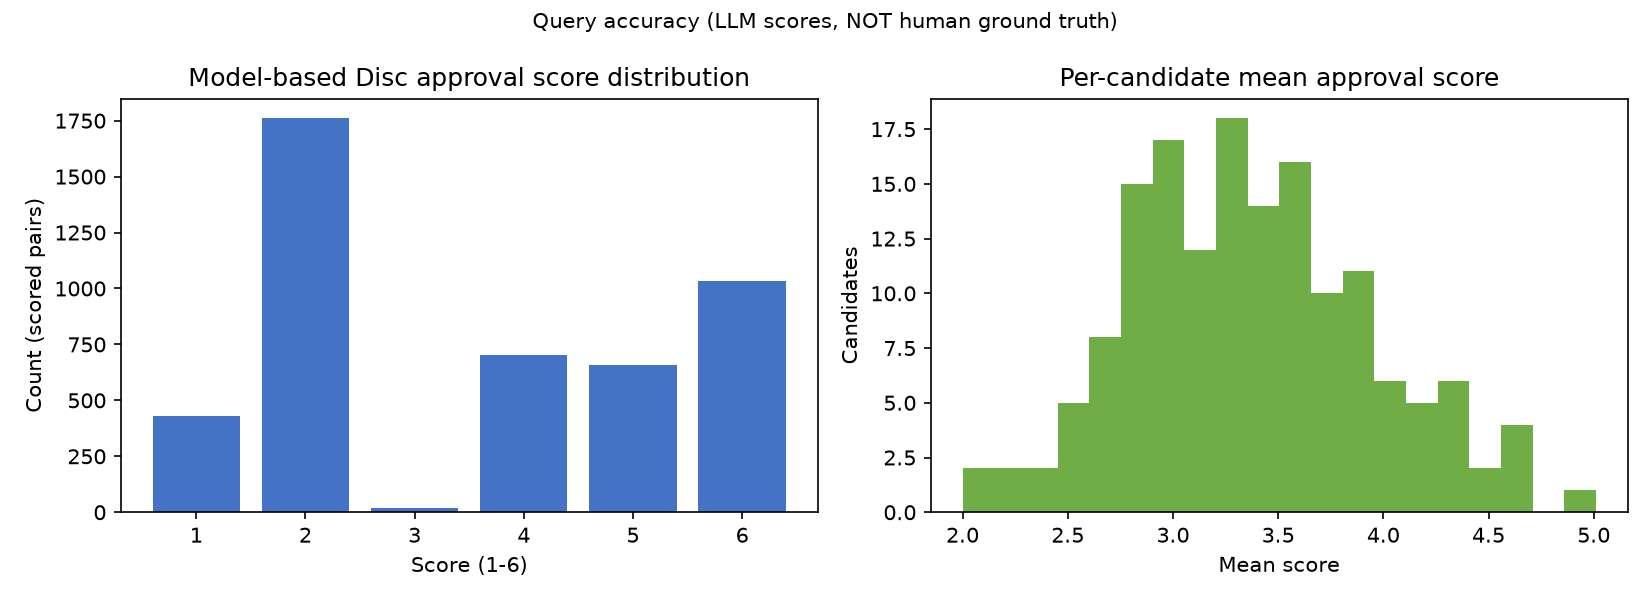
\includegraphics[width=.9\textwidth]{figures/chart_1_query_accuracy.pdf}
\caption{{Distribution of model based approval scores and per candidate mean scores. The left panel shows the count of each score level from 1 to 6, and the right panel shows the distribution of mean scores per candidate.}}
\label{fig:query_accuracy}
\end{figure}

\paragraph{Representation.}
The 18 selected statements assigned a total of 79 distinct participants, giving a coverage of 79.0\%. Each statement received exactly its required support, and the number of assigned participants per statement averages 4.39 with a range from 1 to 7. Figure~\ref{fig:representation} shows both the per statement assignment counts and the split between assigned and remaining participants. The larger groups are associated with longer statements, which command a larger proportional share of the word budget.

\begin{figure}[H]
\centering
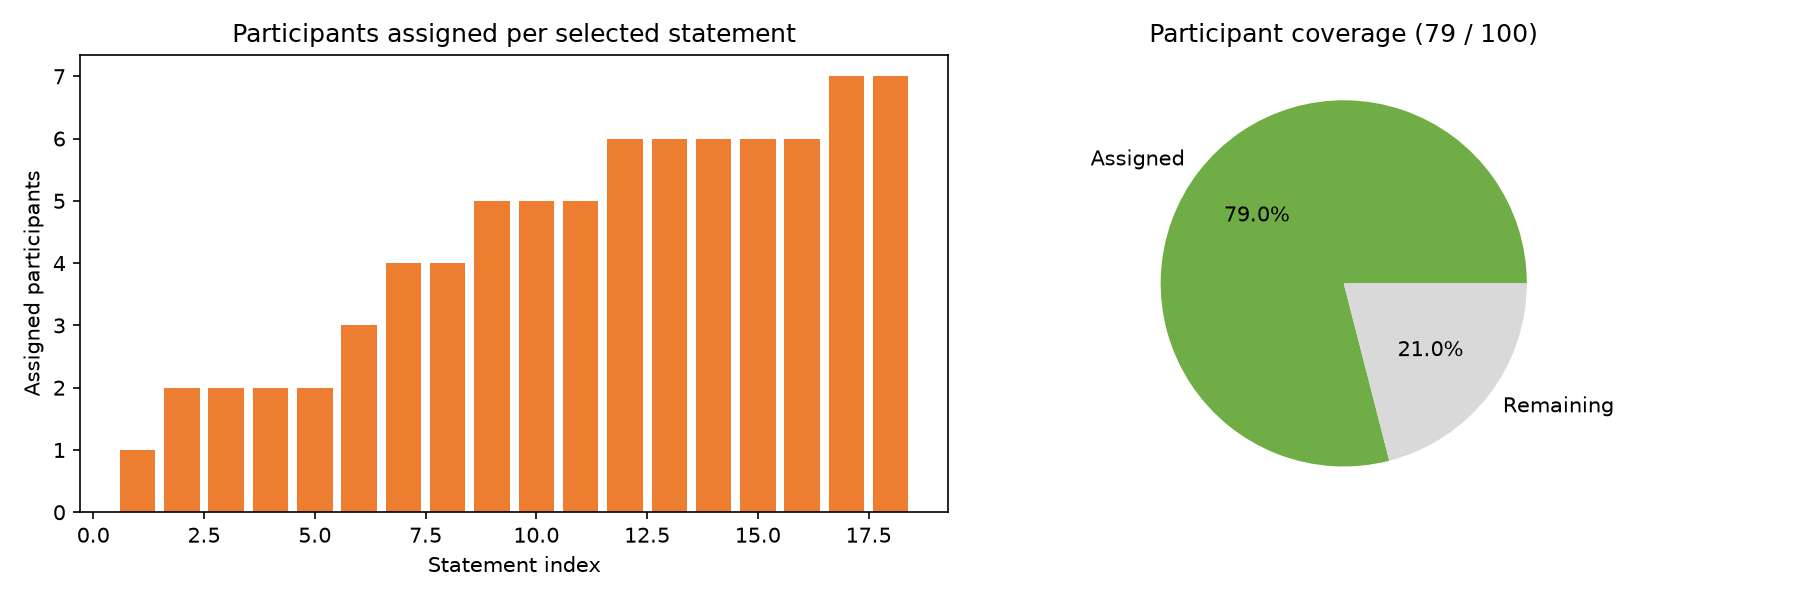
\includegraphics[width=.9\textwidth]{figures/chart_2_representation.pdf}
\caption{{Participant representation. The left panel shows the number of participants assigned to each selected statement, and the right panel shows the split between assigned and remaining participants.}}
\label{fig:representation}
\end{figure}

\paragraph{Statement diversity.}
The selected statements show substantial variation in wording. Table~\ref{tab:diversity} reports the counts of unique statements, the lexical overlap, and the vocabulary and length statistics. Figure~\ref{fig:diversity} complements these summary values by showing the full distribution of pairwise Jaccard similarity and of statement length. The low mean similarity of 0.177 and the spread of word counts from 5 to 33 confirm that the slate covers a wide range of phrasing.

\begin{table}[H]
\centering
\caption{{Summary of statement diversity measures.}}
\label{tab:diversity}
\begin{tabular}{lr}
\toprule
Measure & Value \\
\midrule
Unique selected statements & 16 of 18 \\
Unique generated statements & 154 of 156 \\
Mean pairwise token Jaccard & 0.177 \\
Mean content token Jaccard & 0.140 \\
Type token ratio & 0.366 \\
Mean statement length & 19.9 words \\
\bottomrule
\end{tabular}
\end{table}

\begin{figure}[H]
\centering
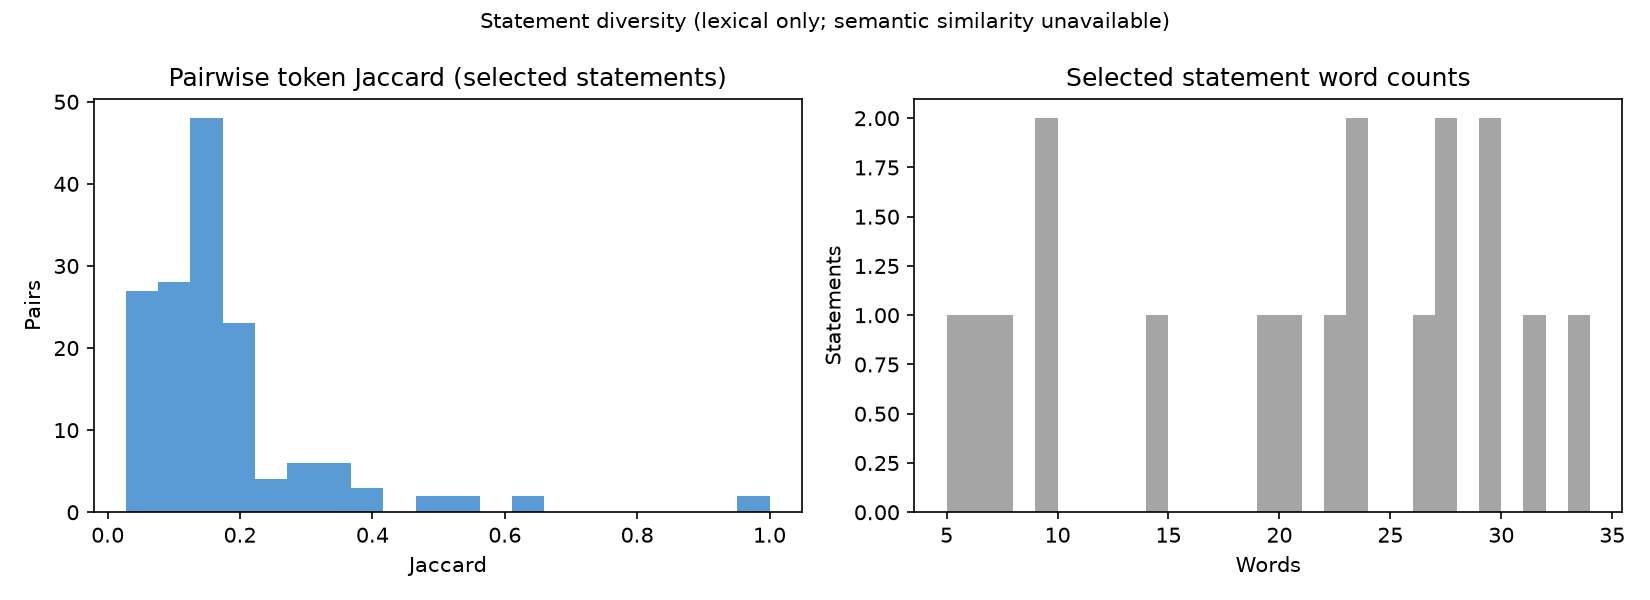
\includegraphics[width=.9\textwidth]{figures/chart_3_diversity.pdf}
\caption{{Statement diversity. The left panel shows the distribution of pairwise token Jaccard similarity among selected statements, and the right panel shows their word count distribution.}}
\label{fig:diversity}
\end{figure}

\paragraph{Budget utilisation.}
The selected statements consume 359 of the 500 available words, corresponding to 71.8\% utilisation, and leave 141 words unspent. The run ended with termination reason \texttt{thresholds\_exhausted}. Figure~\ref{fig:budget} shows the consumed and remaining words and the cumulative growth of the word count after each selection, which rises steadily and ends at the recorded total of 359.

\begin{table}[htb]
\centering
\caption{{Budget utilisation summary.}}
\label{tab:budget}
\begin{tabular}{lr}
\toprule
Measure & Value \\
\midrule
Total budget & 500 words \\
Words consumed & 359 \\
Words remaining & 141 \\
Budget utilisation & 71.8\% \\
Remaining budget share & 28.2\% \\
Selected statements & 18 \\
Termination reason & \texttt{thresholds\_exhausted} \\
\bottomrule
\end{tabular}
\end{table}
\FloatBarrier

\begin{figure}[H]
\centering
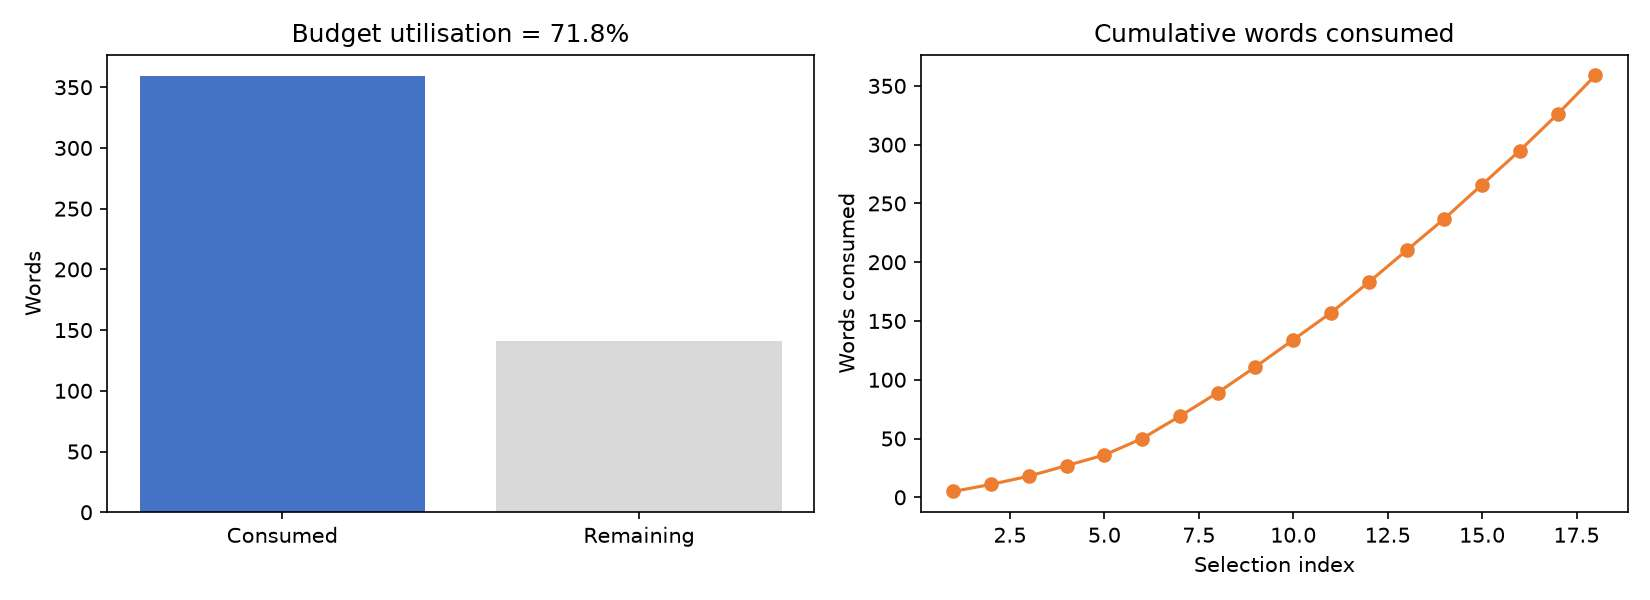
\includegraphics[width=.9\textwidth]{figures/chart_4_budget.pdf}
\caption{{Budget utilisation. The left panel contrasts consumed and remaining words, and the right panel shows the cumulative word count after each selection.}}
\label{fig:budget}
\end{figure}

\paragraph{Runtime.}
The manifest records a total wall clock duration of 2071.93 seconds. Dividing this total by event counts gives 8.26 seconds per candidate record, 13.28 seconds per successful generation, and 115.11 seconds per selected statement. Figure~\ref{fig:runtime} visualises these aggregates. The per statement value is the largest because statements are selected far less often than candidates are generated and scored.

\begin{figure}[H]
\centering
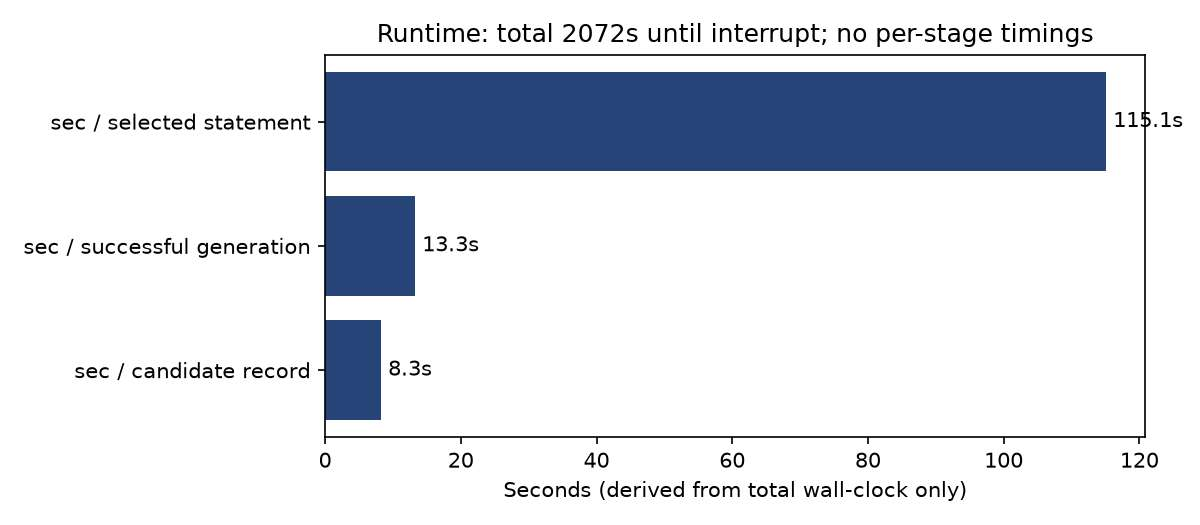
\includegraphics[width=.9\textwidth]{figures/chart_5_runtime.pdf}
\caption{{Runtime aggregates derived from the recorded total wall clock duration. The figure shows seconds per candidate record, per successful generation, and per selected statement.}}
\label{fig:runtime}
\end{figure}

\section{Discussion}

\subsection{Interpretation of Results}

The evaluation describes a pipeline that turns free-text opinions into a budgeted slate of statements. Several patterns in the results are worth interpreting.

First, the approval score distribution shows how the discriminative query uses the 1 to 6 scale. The mean of 3.54 and the median of 4 indicate a general tendency toward moderate or high agreement, while the concentration on levels 2 and 6 shows that the scorer favours the extremes of the scale over the middle. Per candidate means cluster around 3.37, which means that most statements receive different ratings from different participants rather than a uniform score. This is consistent with the role of the discriminative query as a predictor of participant utility~\citep{fish2026gsc,boehmer2025nextgen}. The absence of conflicts between cached and recorded scores shows that the caching layer preserves score values across repeated use.

Second, the representation results show the mechanism by which proportionality is pursued. The 18 selected statements assign 79 distinct participants in balanced groups determined by the admission rule. A statement that attracts more supporters is allocated a larger share of the budget through a larger assigned group, which is the cost aware form of proportional representation described by~\citet{boehmer2025nextgen}. The 21 remaining participants indicate that the search ended while utility levels were still available, rather than through a constraint in the admission rule.

Third, the diversity results show that the slate covers a range of distinct viewpoints. Of the 18 selected statements, 16 are unique. The two repeated statements were admitted in separate rounds, which is permitted because the output slate is a multiset in the original formulation~\citep{fish2026gsc}. The mean pairwise Jaccard similarity of 0.177 and the type token ratio of 0.366 show that the statements use largely distinct vocabulary, supporting the goal of summarising different positions rather than restating a single one.

Fourth, the budget figures show how the word limit shapes the slate. The selected statements consume 359 of the 500 available words, leaving 141 unspent. The budget acts as a cap rather than a target: the process stops when the utility levels are exhausted, which keeps the slate short and readable and matches the motivation for cost aware selection~\citep{boehmer2025nextgen}. The cumulative word count rises steadily across the 18 selections and reconciles exactly with the checkpoint total.

Finally, the runtime figures show where the cost of the experiment lies. The total wall clock duration is 2071.93 seconds, and the derived aggregates give 8.26 seconds per candidate record, 13.28 seconds per successful generation, and 115.11 seconds per selected statement. The largest aggregate is for selected statements because selections occur far less often than candidate evaluations, a pattern also reported for prior LLM based implementations~\citep{boehmer2025nextgen}.

\subsection{Comparison with Relevant Baselines}

The implementation carries out statement selection through a budgeted greedy process. In each round the controller generates candidate statements from the coalitions, scores them with the discriminative query, and keeps the most approved statement. Admission then depends on the cost constrained condition that the number of supporters reaches $\lceil c(\alpha)\,n/B\rceil$. Once a statement is admitted, its highest scoring supporters are assigned to it, removed from the remaining pool, and its word count is deducted from the budget. This realises a cost constrained form of proportional selection in which both the number of supporters and the statement length determine whether a statement enters the slate.

The original generative social choice study of Fish et al.~\citep{fish2026gsc} provides the closest point of comparison, since it uses the same abortion survey and the same two query types. Table~\ref{tab:comparison} contrasts the two systems across the main design choices. Both studies use 100 participants on the topic of abortion policy and rely on discriminative and generative queries. The original work fixes the slate size at $k=5$ and treats statements as having unit cost, whereas our implementation replaces the fixed size with a 500 word budget and measures cost by statement length. The model also differs, with GPT-4o in the original study and a locally served \texttt{qwen3:8b} model here. In the original study, a follow up survey found that 84 of 100 participants felt represented by the selected slate. Our evaluation instead characterises the selected slate directly from the recorded run state, reporting coverage, approval scores, diversity, budget use and runtime.

\begin{table}[htb]
\centering
\caption{{Comparison of the implemented system with the original GSC study of Fish et al.~\citep{fish2026gsc}.}}
\label{tab:comparison}
\begin{tabular}{lll}
\toprule
Aspect & Fish et al.~\citep{fish2026gsc} & This work \\
\midrule
Participants & 100 & 100 \\
Topic & Abortion policy & Abortion policy \\
Query types & Discriminative and generative & Discriminative and generative \\
Model & GPT-4o & Local \texttt{qwen3:8b} \\
Slate control & Fixed size, $k=5$ & 500 word budget \\
Statement cost & Unit cost & Length in words \\
Selection rule & Greedy by $r$-th highest utility & Most approved, then cost constrained admission \\
Representation goal & Balanced justified representation & Cost aware balanced representation \\
Selected output & 5 statements & 18 statements, 16 unique \\
Evaluation & Validation survey with fresh participants & Metrics from the recorded run state \\
\bottomrule
\end{tabular}
\end{table}

The comparison shows that the work preserves the query based selection principle of generative social choice while changing the cost model and the deployment setting. The use of a locally served open weight model makes the pipeline reproducible on ordinary hardware, and the word budget makes the length of the slate an explicit part of the design. The evaluation complements the human validation of the original study with computational measures that describe the quality and cost of the resulting slate.

\section{Conclusion and Future Work}

\subsection{Key Findings}

The central result of this work is a working implementation of cost constrained statement selection on the original abortion survey dataset. The selection process does not simply take the most approved statement: it first identifies the statement with the largest supporter set, then checks whether those supporters can cover the statement's proportional share $\lceil c(\alpha)\,n/B\rceil$ of the word budget. Only statements that satisfy this condition are admitted, and the participating supporters are assigned in balanced groups and removed from the pool. This best then qualify rule, combined with word based costing, is the main improvement over fixed size slate selection, because it lets the budget decide both how many statements are selected and how much of it each statement receives.

The experiment demonstrates this mechanism end to end. From 251 generated candidates, the process selected 18 statements representing 79 of the 100 participants while consuming 359 of the 500 available words. The run ended when the utility levels were exhausted, with 141 words left unspent, showing that the budget acts as a cap rather than a fixed target. The admission rule allocated each statement only its required support, so longer statements drew larger balanced groups, which is how cost aware proportionality is realised in practice.

The supporting measurements confirm that the process behaved consistently. The discriminative query produced 4603 approval scores, the selected statements showed 16 unique texts with low lexical overlap, and all 16 reconciliation checks passed. These results show that a locally served open weight model can implement the query based selection process and that the cost constrained admission rule produces a coherent, budgeted slate on the abortion survey data. The feasibility of this selection mechanism, rather than the descriptive figures alone, is the principal finding of the work.

\subsection{Contributions}

The contributions of this work are as follows.

\begin{itemize}
\item A complete implementation of the cost constrained statement selection process on the original abortion survey dataset. The selection logic follows the best then qualify rule: at each round the most approved candidate is identified and admitted only if its supporters meet the proportional requirement $\lceil c(\alpha)\,n/B\rceil$. Assigned supporters are the highest scoring agents and are removed from the pool, so each statement represents a balanced group. \smallskip

\item A slate design governed by an explicit word budget instead of a fixed number of statements. Statement cost is measured by a whitespace token count, and the budget is reduced by each admitted statement. This lets the budget determine both how many statements are selected and how much of it each statement receives, in contrast to unit cost selection. \smallskip

\item A query layer implemented with a locally served open weight model. Both the discriminative and generative queries use \texttt{qwen3:8b} through Ollama, with validated generation output, integer approval scores from 1 to 6, and a score cache for repeated participant statement pairs, making the pipeline reproducible without a proprietary API. \smallkip

\item An evaluation of the resulting slate from the recorded run state, covering approval scores, participant coverage, statement diversity, budget utilisation and runtime, together with reconciliation checks that verify the internal consistency of assignments, counts and budget totals.
\end{itemize}

Together these contributions connect the formal design of cost constrained generative social choice to a working, inspectable implementation on a real survey dataset.

\subsection{Limitations}

The following points define the scope of the evaluation and should be read alongside the results. \smallskip

\begin{itemize}
\item The evaluation is based on the state recorded during a single run of the process. The reported figures describe the slate produced by that run, and a full sweep over multiple budgets would be needed to characterise how the selection rule behaves across different budget levels. \smallskip

\item Approval scores are generated by the language model and describe its estimate of participant agreement. The evaluation therefore reports the distribution and internal consistency of these scores, and any comparison with human ratings would require a separate validation survey. \smallskip

\item Statement diversity is measured lexically, through token overlap, unique texts and type token ratio. Capturing semantic similarity would require embeddings of the generated statements. \smallskip

\item Runtime is recorded as a single wall clock duration in the manifest. The derived per event figures are aggregates computed from that total, since the run state does not contain separate timestamps for generation and scoring. \smallskip

\item The study is positioned at an empirical, descriptive level. It measures what the implemented process produced and verifies internal consistency, but it does not establish a theoretical representation guarantee for the resulting slate.
\end{itemize}

These boundaries keep the claims aligned with the evidence available from the experiment, while leaving clear directions for further development.

\subsection{Future Improvements}

Several directions extend the work reported here. \smallskip

\begin{itemize}
\item Run the process across multiple word budgets, for example 250, 500, 1000 and 2000 words, and compare how the selection rule allocates budget and assigns participants at each level. This would show how the cost constrained admission rule behaves as the budget grows. \smallskip

\item Add a human validation survey in which fresh participants rate the selected statements. This would allow the agreement scores produced by the model to be compared with human ratings, in the same spirit as the validation step of the original study~\citep{fish2026gsc}. \smallskip

\item Compute embeddings of the generated statements and measure semantic similarity between them. This would complement the lexical overlap measures with a view of how closely the statements express the same meaning. \smallskip

\item Record separate timestamps for generation and scoring calls. This would replace the aggregate runtime figures with measured per stage timings and make the cost of each query type explicit. \smallskip

\item Extend the query layer to other open weight models and compare their agreement scores, generation success rates and runtimes on the same dataset. This would show how sensitive the slate is to the choice of local model. \smallskip

\item Apply the same implementation to other opinion datasets, so that the cost constrained selection process can be evaluated beyond the abortion survey.
\end{itemize}

Each of these extensions builds directly on the pipeline implemented here and would deepen the empirical evidence for cost constrained generative social choice.

\begin{thebibliography}{999}

\bibitem{aziz2017jr}
Aziz, H., Brill, M., Conitzer, V., Elkind, E., Freeman, R., and Walsh, T. (2017). Justified Representation in Approval-Based Committee Voting. \emph{Social Choice and Welfare}, 48(2), pp. 461 to 485. arXiv:1407.8269.

\bibitem{boehmer2025nextgen}
Boehmer, N., Fish, S., and Procaccia, A. D. (2025). Generative Social Choice: The Next Generation. \emph{arXiv preprint} arXiv:2505.22939.

\bibitem{fish2026gsc}
Fish, S., G\"olz, P., Parkes, D. C., Procaccia, A. D., Rusak, G., Shapira, I., and W\"uthrich, M. (2026). Generative Social Choice. \emph{Journal of the ACM}, 73(2), Article 11. doi:10.1145/3799709.

\bibitem{gsc_survey_data}
Generative Social Choice Survey Data (2024). Available online: \url{https://github.com/generative-social-choice/survey_data/} (accessed on 17 November 2026).

\bibitem{ollama2026}
Ollama (2026). \emph{Ollama: Run Large Language Models Locally}. Available online: \url{https://github.com/ollama/ollama} (accessed on 17 November 2026).

\bibitem{yang2025qwen3}
Yang, A., Li, A., Yang, B., Zhang, B., Hui, B., Zheng, B., Yu, B., et al. (2025). Qwen3 Technical Report. \emph{arXiv preprint} arXiv:2505.09388.

\end{thebibliography}

\appendix 

\include{appendix}

\end{document}
